\chapter{Diseño de la interfaz gráfica.}\label{chap:GUI}
\epigraphhead [30]{%
  \epigraph{``Desde el punto de vista de un programador, el usuario no es más que un periférico que teclea cuando se le envía una petición de lectura"}%
  {Peter Williams.}%
}
 
 
	El extremo final del ``puente'' es la interfaz gráfica donde el usuario final operará con el programa. En este capítulo se detalla el diseño de la misma.
	
	\section{Disposición de los elementos en la ventana principal.} \label{sec:gui_mainframe}
	Se ha diseñado una ventana principal con barras de herramientas y de estado donde colocar los elementos. La gráfica donde se visualizarán los datos es una parte fundamental del programa, por lo que se decidió que ocupara dos tercios del espacio disponible verticalmente y el tercio restante lo ocuparán los controles para la adquisición de datos, visualización de los mismos y otras opciones no relacionadas con la gráfica. La resolución con la que se ha creado el diseño es 1024x768; una resolución modesta pero segura, pues cualquier monitor antiguo es capaz de mostrarla. Pese a que algunos test se han realizado bajo 1280x1024 o incluso panorámico a 1920x1080 se ha asegurado que la visualización de los componentes sea óptima a 1024x768. 
	
	\subsection{Los dos tercios superiores.}\label{sec:gui_graph}
		Debajo de la gráfica se ha incluido una pequeña barra de herramientas, a la izquierda para controlar elementos de la gráfica como el zoom, mover la misma o exportar el dibujo, mientras que a la derecha se han incluido otros controles como una barra deslizante para elegir la tasa de refresco automático de los datos, un botón para desactivarla, un botón para comenzar y otro para detener la adquisición de todos los canales disponibles, y un botón para actualizar los datos de la gráfica manualmente. 

	El resultado final se puede apreciar en la \autoref{fig:gui-graph_sample}.
\begin{figure}[hb]
  \centering
  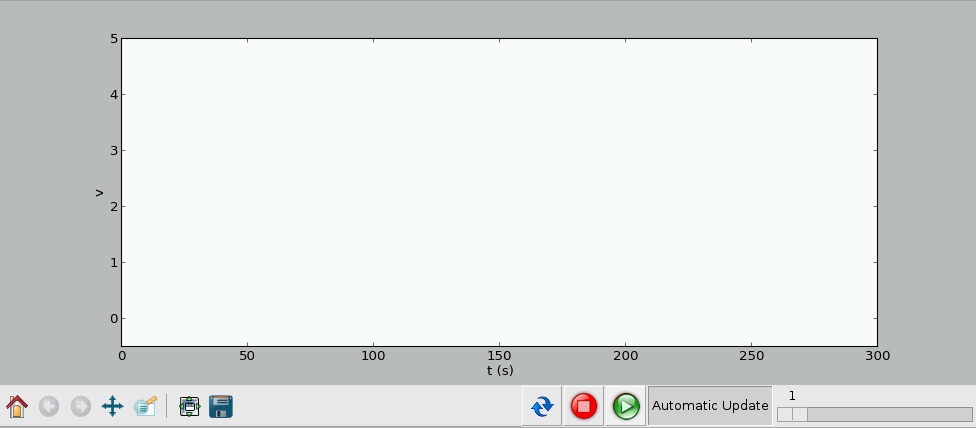
\includegraphics[width=1\textwidth]{img/gui-graph_sample.png}
  \caption[El conjunto de la gráfica y sus controles en nuestro programa.]{El conjunto de la gráfica y sus controles.}
  \label{fig:gui-graph_sample}
\end{figure}

\subsection{Tercio inferior de la ventana principal.}
	Para dividir los controles de la adquisición, la visualización de los datos y la exportación de los mismos (estas serán las opciones por el momento) se han creado tres pestañas:
	
	\subsubsection{Control de adquisición de datos.}\label{sec:gui_AcquisitionGUI}
	La primera pestaña, correspondiente a los controles de adquisición de datos se ha dividido horizontalmente en cuatro columnas, una por cada canal. 
	
	La implementación se ha realizado de manera que cada columna contiene un objeto AcquisitionGUI representando un panel con los siguientes controles:
\begin{itemize}
	\item Un texto informativo de estado del módulo de adquisición de datos junto con un indicador de colores.
	\item Un desplegable que permite elegir el color de la línea que se dibujará en la gráfica.
	\item Un cuadro de texto donde especificar la frecuencia de muestreo a la que se desea que trabaje el canal.
	\item Un botón para ``Stop'' para detener la adquisición de datos y otro ``Start'' para comenzar la misma.
	\item Un botón ``Simulation'' para cargar en ese canal el módulo de simulación en lugar del módulo de adquisición de datos en tiempo real.
\end{itemize}
	Cada uno de estos paneles está relacionado con un módulo de adquisición de datos si está disponible y el control del mismo así como la disposición de los datos para la gráfica se realiza directamente desde aquí. 
	
	El constructor de la clase incluye el número de canal al que va a representar y que inicializará a través del interfaz piDA. De esta manera es posible aumentar la cantidad de canales a los que da soporte el programa tan solo creando más paneles, ya que todas las funciones relacionadas están dentro del mismo.
	
	El resultado final se puede apreciar en la \autoref{fig:gui-acq_sample}.
	
\begin{figure}[hc]

  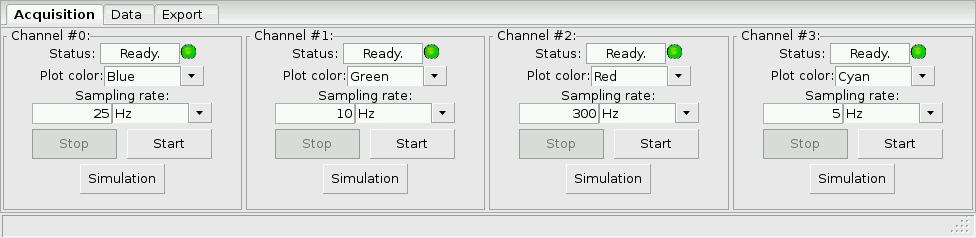
\includegraphics[width=1\textwidth]{img/gui-acq_sample.png}
  \caption{Pestaña para controlar las adquisiciones de datos.}
  \label{fig:gui-acq_sample}
\end{figure}
%	\pagebreak
	\subsubsection{Visualización de datos.}\label{sec:gui_DataGUI}
	La segunda pestaña corresponde a la visualización de datos donde los datos son mostrados directamente como su valor \emph{x} (tiempo) e \emph{y} (voltaje en este prototipo). El diseño del panel formado por cinco columnas es el siguiente:
\begin{itemize}
	\item Una columna con cinco botones cuadrados, cada uno con un diseño personalizado especificando su función. El primero actualizará los datos de todas las tablas, el segundo los datos de la tabla correspondiente al primer canal, el tercero los datos de la tabla correspondiente al segundo canal, el cuarto los del tercer canal y el quinto los del cuarto canal.
	\item Cuatro columnas con cuatro tablas de dos columnas cada tabla para los datos de cada canal, rellenadas bajo petición del usuario por los botones de la columna anterior.
	
	Las tablas han sido modificadas en una subclase interna ya que el control que provee WxPython no permite ajustar el tamaño de las columnas de datos.  De esta manera el control una vez creado ajusta el tamaño de las columnas al espacio disponible.
\end{itemize}
	Se ha decidido liberar de carga al procesador y que la actualización de los datos de las tablas se realice mediante petición expresa del usuario con los botones de la primera columna. Se ha creado un diseño para cada uno de los botones con Adobe Fireworks\cite{adobe_fireworks} para que ocupen el mínimo espacio posible al carecer de texto pero siga siendo intuitiva su función.

	La modularización de este panel es una tarea pendiente.
	
	En la \autoref{fig:gui-data_sample} se puede ver el resultado final.
	
\begin{figure}[hb]
  \centering
  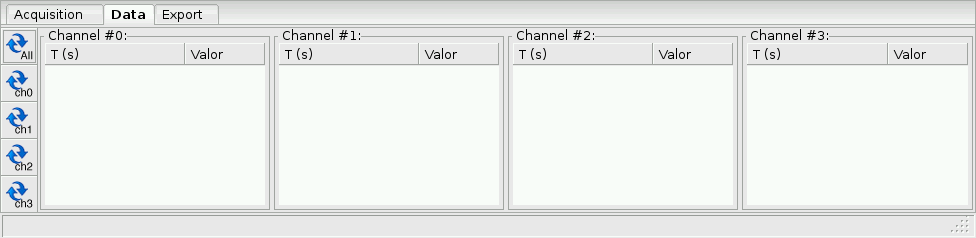
\includegraphics[width=1\textwidth]{img/gui-data_sample.png}
  \caption{Pestaña de visualización de datos.}
  \label{fig:gui-data_sample}
\end{figure}	
	\pagebreak
	\subsubsection{Exportación de datos.}\label{sec:gui_ExportGUI}
	Por último, la tercera pestaña correspondiente a la exportación de datos consiste en dos filas principalmente:
\begin{itemize}
	\item Una primera fila formada por cuatro columnas, cada una de ellas representando cada canal. Dentro de cada columna se han añadido campos de texto para personalizar el título de la exportación, la etiqueta del eje X, la etiqueta del eje Y y sendos botones para exportar los datos en formato CSV y PDF.
	\item La segunda fila se ha utilizado para exportar datos de varios canales a la vez a un único fichero. Se han incluido cuatro \emph{checkboxes} para seleccionar los canales que se exportarán al fichero, una lista desplegable para truncar los valores de tiempo a segundos, milisegundos, microsegundos o nanosegundos y sendos botones para exportar a CSV a PDF.
\end{itemize}
	
	El exportado de datos a PDF no está implementado en esta versión, y al igual que el anterior panel, éste tampoco ha sido modularizado.
	
	El resultado final: \autoref{fig:gui-export_sample}.
	
\begin{figure}[hb]
  \centering
  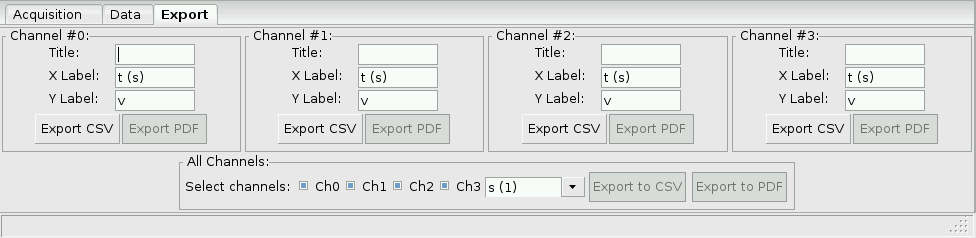
\includegraphics[width=1\textwidth]{img/gui-export_sample.png}
  \caption{Pestaña de exportación de datos.}
  \label{fig:gui-export_sample}
\end{figure}	
\pagebreak
\section{Resultado final.}
El conjunto de los anteriores elementos forman la ventana principal del programa dando una apariencia sobria y un control intuitivo sobre las funciones.
\begin{figure}[h]
  \centering
  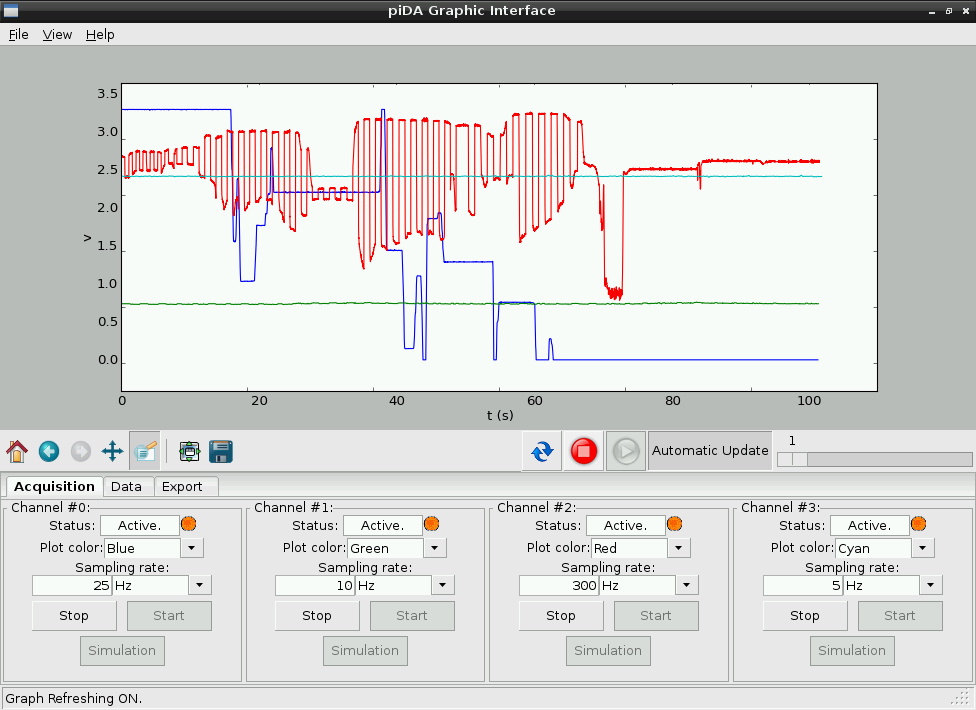
\includegraphics[width=1\textwidth]{img/pida_4ch_sample.png}
  \caption{El interfaz gráfico de nuestro programa.}
  \label{fig:gui-full_sample}
\end{figure}	